\documentclass{article}

% Geometry and layout
\usepackage[a4paper, total={7in, 10in}]{geometry}

% Math packages
\usepackage{amsmath, amssymb, amsthm, mathtools}
\usepackage{mathrsfs} 
\usepackage{bm} 

% Theorem environments
\newtheorem{theorem}{Theorem}
\newtheorem{proposition}{Proposition}
\newtheorem{lemma}{Lemma}
\newtheorem{corollary}{Corollary}
\newtheorem{definition}{Definition}
\newtheorem{example}{Example}
\newtheorem{remark}{Remark}

% References and Citations
\usepackage{hyperref}
\usepackage[capitalize,nameinlink]{cleveref}

% Lists and structuring
\usepackage{enumitem}

% Figures and Tables
\usepackage{graphicx, float}
\usepackage{caption, subcaption}
\usepackage{booktabs}

% Algorithms
\usepackage{algorithm}
\usepackage{algpseudocode}

% Colors for emphasis
\usepackage{xcolor}

% TikZ for diagrams
\usepackage{tikz}
\usetikzlibrary{arrows.meta, positioning, calc}

%fig shortcut
\newcommand{\fig}[2]{
    \begin{figure}
        \centering
        \includegraphics[width=\textwidth]{#1}
        \caption{#2}
        \label{fig:#1}
    \end{figure}
}

\setlength{\parindent}{0pt}

\title{Computer Vision for Automated Driving}
\author{Elias W.J. Müller}
\date{FS26}

\begin{document}

\maketitle

\tableofcontents
\newpage

\section{Part I: Fundamentals}
\subsection{Definitions}
\begin{definition}[Computer Vision]
Inverse algorithmic process to infer properties of the world based on sensory observations.
\end{definition}
\begin{definition}[Autonomous Car (ADS-DV)]
ADS-equipped vehicle designed for driverless operation within its given operational design domain.
\end{definition}
\begin{definition}[Automated Driving System (ADS)]
Hardware and software collectively capable of performing the entire DDT on a sustained basis, possibly limited to a specific ODD.
\end{definition}
\begin{definition}[Operational Design Domain (ODD)]
Conditions (environmental, geographical, temporal, traffic/roadway) under which a given ADS is designed to function.
\end{definition}
\begin{definition}[Dynamic Driving Task (DDT)]
All real-time operational and tactical functions for on-road driving (excludes strategic functions). Subtasks: (1) lateral control, (2) longitudinal control, (3) OEDR monitoring, (4) OEDR execution, (5) maneuver planning, (6) conspicuity enhancement.
\end{definition}
\begin{definition}[OEDR]
Object and Event Detection and Response. DDT subtasks 3--4: monitor driving environment via detection, recognition, classification, response preparation, and response execution.
\end{definition}
\begin{definition}[Driving Automation System]
Hardware and software capable of performing part or all of the DDT. $\text{ADS} \subseteq \text{Driving Automation Systems}$. Four core modules: (1) semantic and geometric \textbf{Perception} (2) \textbf{Prediction} from temporal perception (3) path and motion \textbf{Planning} via response determination (4) \textbf{Control}
\end{definition}

\begin{figure}
    \centering
    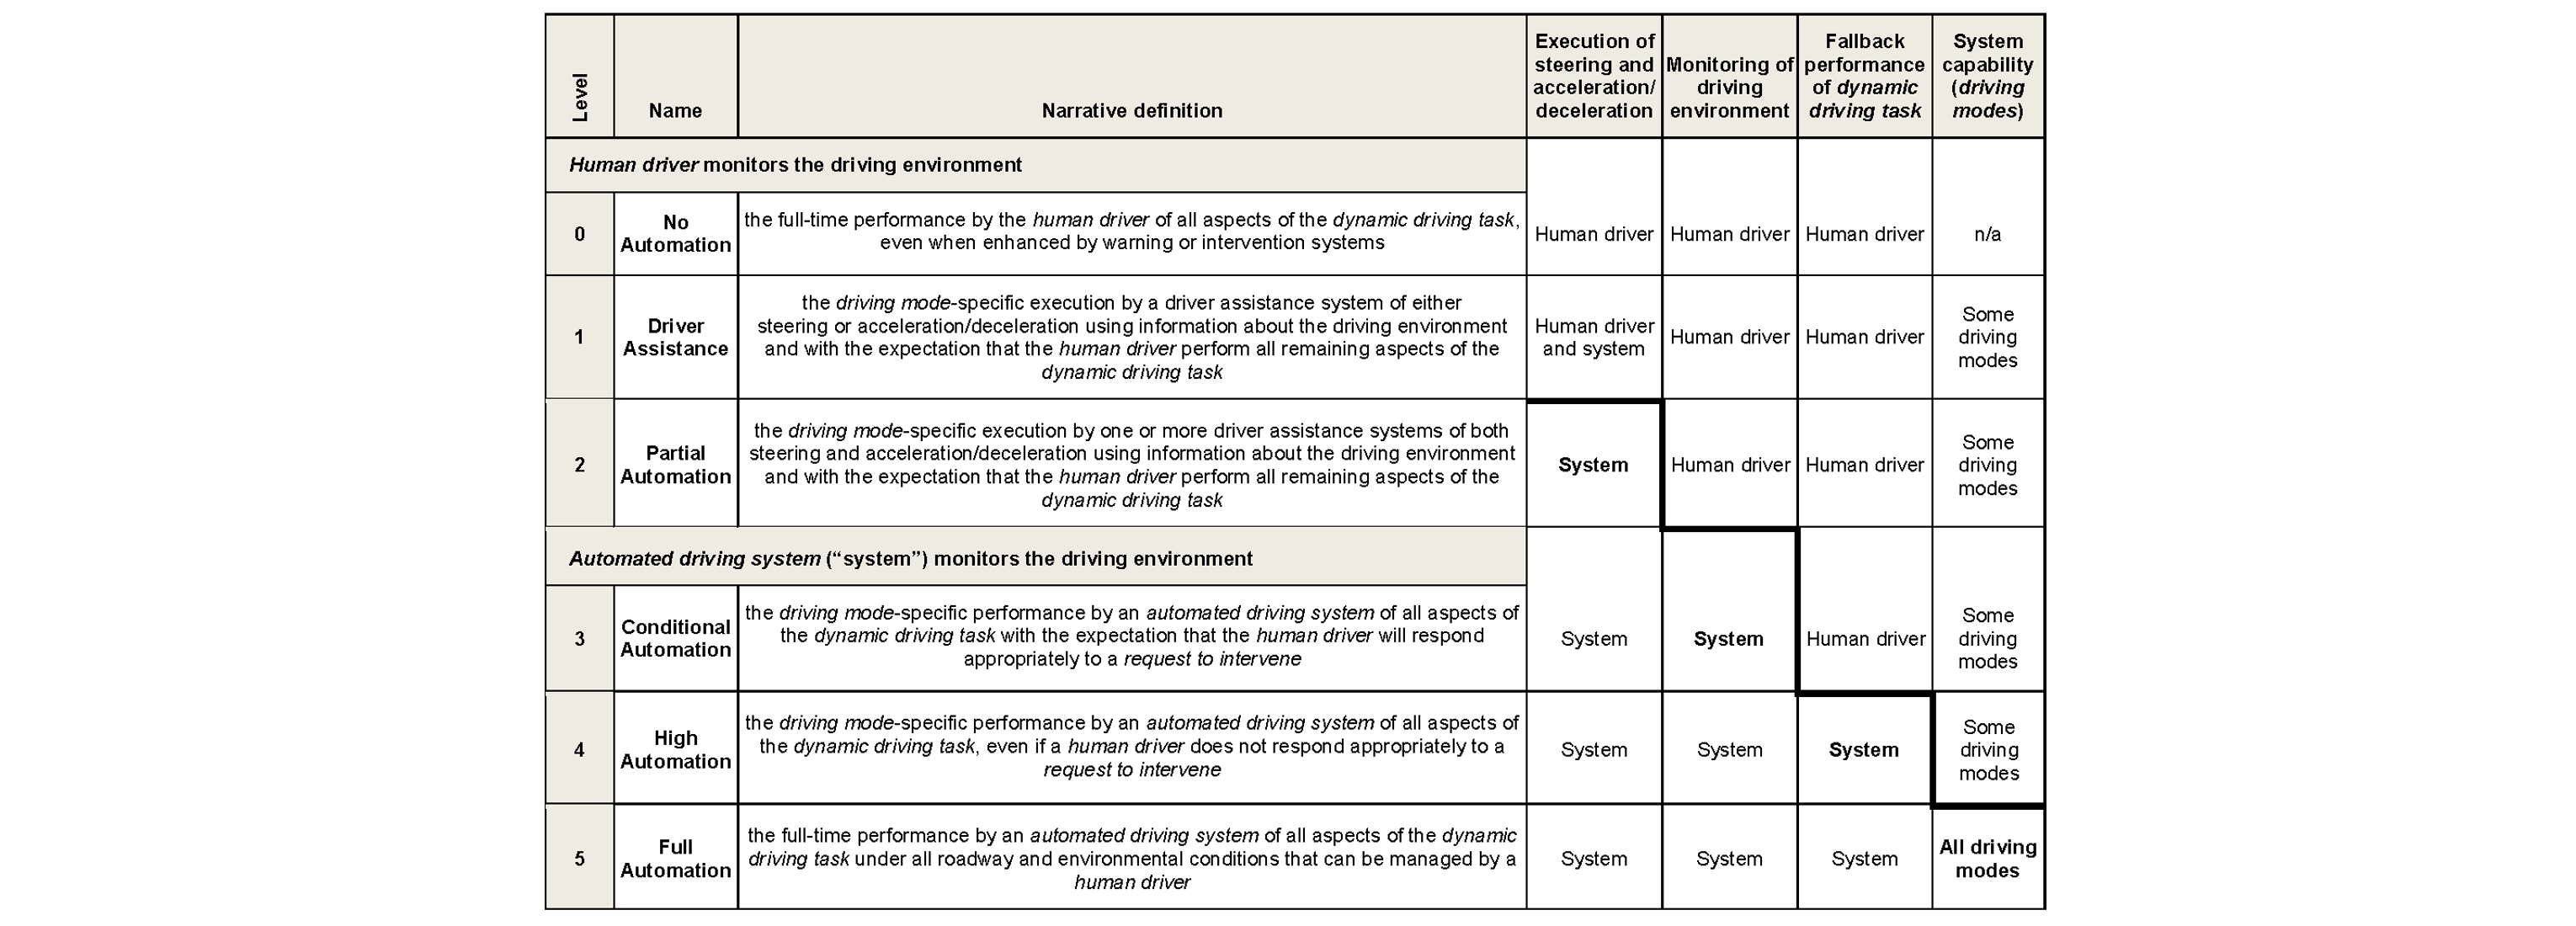
\includegraphics[width=\linewidth]{img/SAE_Levels.png}
    \caption{SAE levels of driving automation}
    \label{fig:SAE_Levels}
\end{figure}

\subsection{Optical Autonomous Driving Sensors}
Countless sensor choices exist. We make the distinction of \textbf{external} (\textit{camera, lidar, radar, event camera, GPS, IMU, speedometer, ...}) and \textbf{internal} (\textit{camera, thermal camera, microphone}) sensors. Our focus further lies on the \textit{Optical Sensors}.\\

Optical Sensors can be categorized along the following features: 
\begin{itemize}
\item \textit{Wavelength}: spectral band of light the sensor operates in (e.g.\ visible, near-infrared, millimeter-wave).
\item \textit{Active or Passive}: whether the sensor emits its own signal (active) or relies on external illumination (passive).
\item \textit{Resolution}: spatial density of measurements; determines fineness of detail captured.
\item \textit{Latency / Frame Rate}: temporal frequency at which full measurements are acquired.
\item \textit{Field of View} (FOV): angular extent of the observable scene, horizontal and vertical.
\item \textit{Range}: maximum distance at which the sensor can reliably detect objects.
\end{itemize}

\subsubsection{Light Detection and Ranging (Lidar)}
\textbf{Characteristics}: Active sensor, near-infrared wavelength (905nm), direct range measurements via time of flight (TOF), i.e., timing of light emission until recapture of photons, large horizontal and fair vertical FOV (3D), fair resolution

\paragraph{Pulsed Lidar}
Multiple short laser pulses emitted in different directions and at different times. Each measurement: pulse emitter $\to$ beam steering $\to$ target $\to$ photodetector (APD). A timer measures the round-trip delay to infer range $R_0$

\begin{figure}[H]
    \centering
    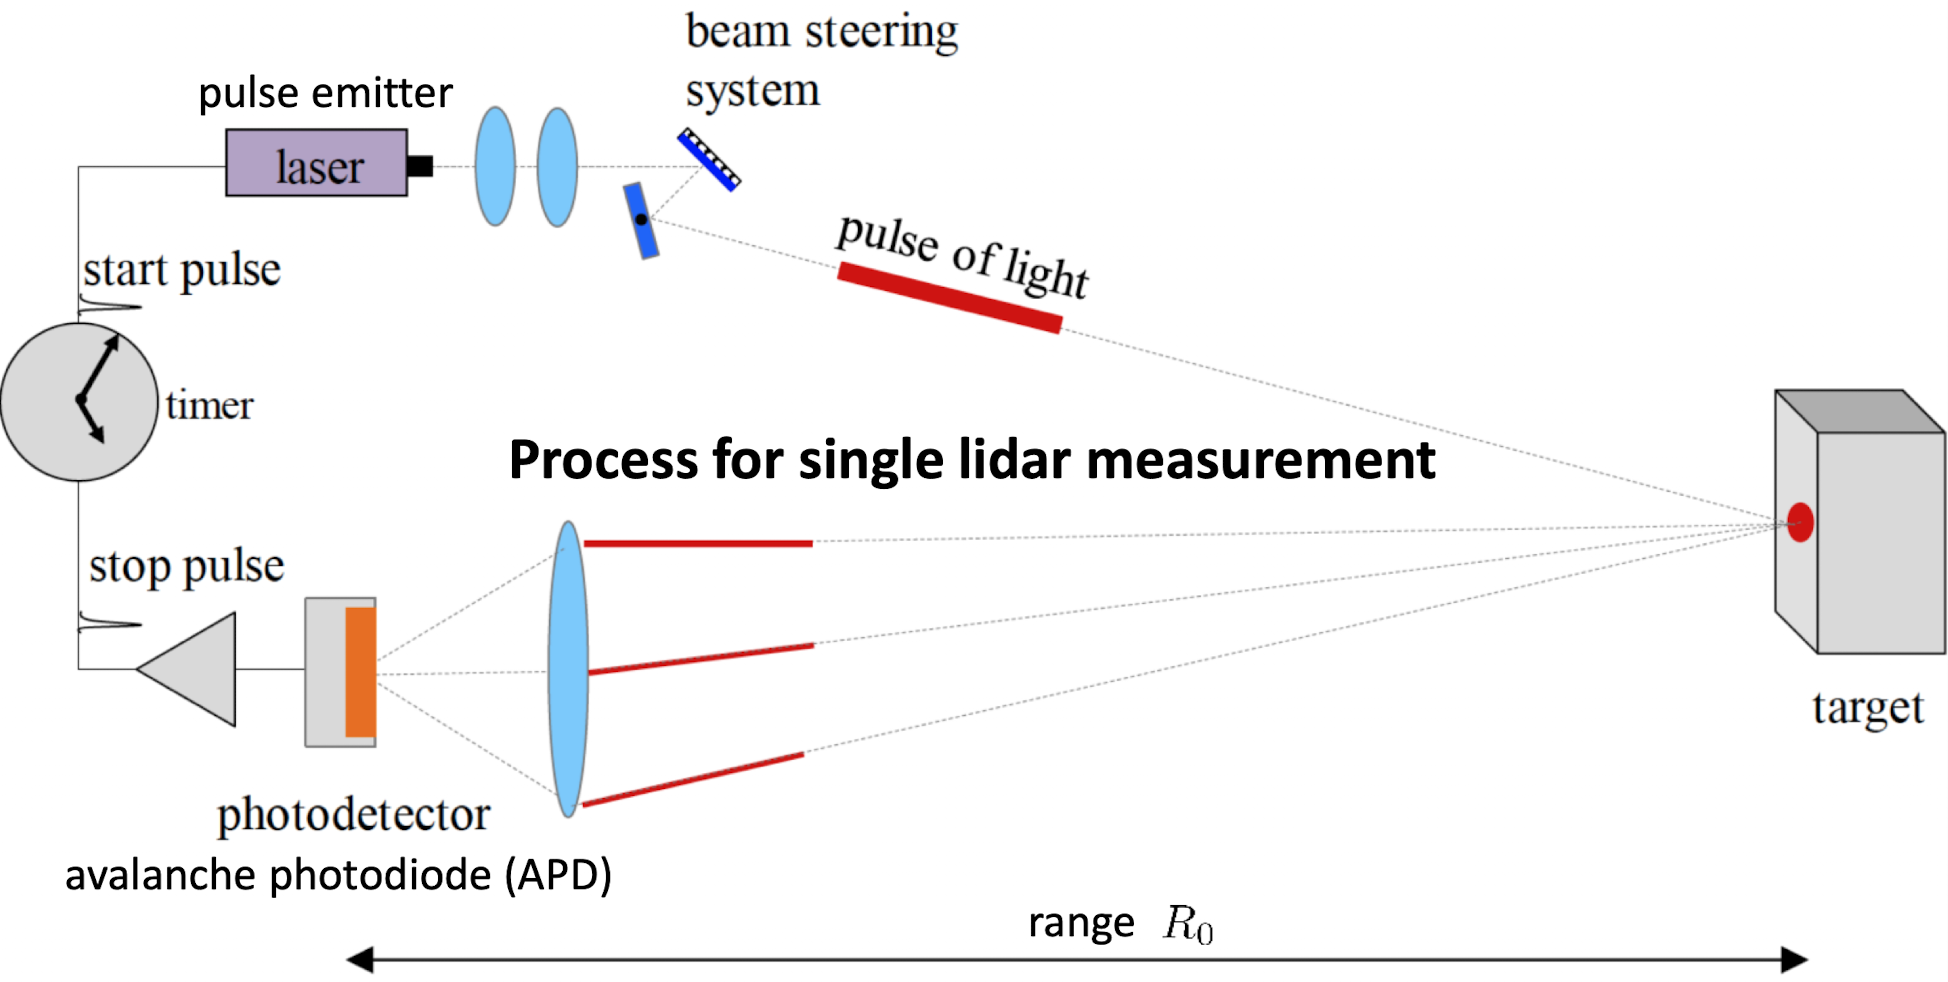
\includegraphics[width=0.6\linewidth]{img/lidar.png}
    \caption{Lidar working principle}
    \label{fig:lidar}
\end{figure}

\subparagraph{Beam Configurations.}
Real beams diverge; receivers have finite FOV. Two configurations:
\begin{itemize}
    \item \textit{Coaxial}: transmitter and receiver share a common optical axis.
    \item \textit{Bistatic}: optical axes of transmitter and receiver are parallel but offset.
     The \textbf{crossover function} $\xi(R) \in [0,1]$ gives the fraction of the illuminated area observed by the receiver as a function of range. For bistatic: $\xi(R)=0$ at short range (no crossover), $\xi(R)=1$ beyond some $R_2$ (full crossover).
\end{itemize}

\subparagraph{Pulse Waveform (Sinusoidal Form).}
\begin{equation*}
    P_T(t) = \begin{cases} P_0 \sin^2\!\left(\dfrac{\pi}{2\tau_H}\, t\right), & 0 \leq t \leq 2\tau_H, \\ 0, & \text{otherwise.} \end{cases}
\end{equation*}
where $P_T(t)$: emitted radiant power, $P_0$: peak power, $\tau_H$: half-power pulse width ($10$--$20$\,ns), $c\tau_H$: spatial half-power width ($3$--$6$\,m).\\
Physically more realistic is the square-exponential form (left heavy, right tailed) -- omitted here. 

\subparagraph{Linear System Model.}
Received radiant power as a convolution of emitted power with the optical system impulse response:
\begin{equation*}
    P_R(R) = C_A \int_0^{2R/c} P_T(t)\, H\!\left(R - \frac{ct}{2}\right) dt
\end{equation*}
where $P_R(R)$: range-dependent received power, $H(R)$: impulse response of the optical system, $C_A$: system constant (independent of time and range). $ct/2$ maps time $t$ to the corresponding range (round-trip).
 
\textbf{Intuition:} $H(R)$ is what we would receive from a perfectly concentrated (Dirac) pulse; the actual response is a smeared version due to finite pulse width - ambiguity from temporal profile/ early or late photon.

\subparagraph{Impulse Response Decomposition.}
\begin{equation*}
    H(R) = H_C(R)\, H_T(R)
\end{equation*}
\begin{itemize}
    \item \textit{Optical channel}: $H_C(R) = \dfrac{T^2(R)}{R^2}\,\xi(R)$, \quad where $T(R) = \exp(-\alpha R)$ is the one-way transmission loss ($\alpha$ depends on visibility, assumes homogeneous scattering medium).
    \item \textit{Target}: $H_T(R) = \rho_0\,\delta(R - R_0)$ in clear weather, where $\rho_0$ is the differential reflectivity.
\end{itemize}
 
\subparagraph{Clear Weather Simplification.}
With $\alpha = 0$ (no attenuation -- clear air) and $\xi(R_0)=1$:
\begin{equation*}
    H(R) = \frac{1}{R_0^2}\,\rho_0\,\delta(R - R_0)
\end{equation*}
Substituting into the linear system model yields:
\begin{equation*}
    P_R(R) = \begin{cases} \dfrac{C_A P_0 \rho_0}{R_0^2}\, \sin^2\!\left(\dfrac{\pi(R-R_0)}{c\tau_H}\right), & R_0 \leq R \leq R_0 + c\tau_H, \\ 0, & \text{otherwise.} \end{cases}
\end{equation*}
 
\textbf{Intuition:} The target acts as a Dirac delta in range, so the convolution merely shifts and scales the emitted waveform — the received pulse preserves the shape of $P_T$, centered at $R_0$. The $1/R_0^2$ decay is the inverse-square law: emitted power spreads over a sphere of area $\propto R_0^2$. The proportionality to $\rho_0$ is why lidar returns per-point \textit{intensity} alongside range. The pulse occupies a range interval of width $c\tau_H$, so shorter pulses yield finer range resolution at the cost of less energy per pulse.

\subparagraph{Features of Pulsed Lidar.}
\begin{itemize}
    \item \textit{Ranging precision}: limited by temporal resolution of timing electronics. Typical $\sim 0.1$\,ns $\Rightarrow$ $\sim 1.5$\,cm.
    \item \textit{Maximum range}: limited by signal to noise ratio (SNR) (attenuation + detector noise/jitter): $100$--$200$\,m.
    \item \textit{Range--rate trade-off}: maximum unambiguous range is inversely proportional to pulse repetition rate (aliasing) -- upper limit of the integral
\end{itemize}

\subparagraph{Acquisition of 3D Point Clouds.}
Each pulse yields a single range measurement along a direction $(\alpha, \epsilon)$. To obtain a 3D point cloud, the sensor scans across a range of azimuth $\alpha$ and elevation $\epsilon$ values, which jointly define the FOV. Spherical-to-Cartesian conversion:
\begin{equation*}
    \begin{bmatrix} x \\ y \\ z \end{bmatrix}
    = \mathbf{h}^{-1}(r, \alpha, \epsilon)
    = \begin{bmatrix} r \cos\alpha \cos\epsilon \\ r \sin\alpha \cos\epsilon \\ r \sin\epsilon \end{bmatrix}
\end{equation*}
Each point additionally carries an \textit{intensity} value $= f(P_R(R_0))$, derived from the peak received power.
 
\subparagraph{Scanning Mechanisms.}
Taxonomy: non-scanning (flash) vs.\ scanning lidar. Scanning subdivides into non-mechanical (OPA, solid-state) and mechanical (MEMS, motorized optomechanical). Driving-relevant types are motorized mechanical and MEMS scanners.\\
 
\textit{Motorized mechanical}: nodding-mirror tilt controls vertical FOV; rotating housing ($>1000$ RPM) provides panoramic $360^\circ$ horizontal FOV. Modern systems use laser/photodiode arrays $\Rightarrow$ mechanical rotation only along azimuth. Horizontal angular resolution up to $0.1^\circ$, max range up to $200$\,m. \\
 
\textit{MEMS}: tiny oscillating mirrors (few mm diameter) steer individual pulses. 1D MEMS scans one angular dimension (needs laser array or motor for the other); 2D MEMS scans both. Resonant scanning: frequency $=$ resonant frequency of mirror, high frame rate, sensitive to environmental variation. Non-resonant: more robust, lower frame rate.
 
\begin{center}
\begin{tabular}{l|l}
    \textbf{Motorized Mechanical} & \textbf{MEMS} \\ \hline
    Panoramic $360^\circ$ horizontal FOV & Limited ($\sim 120^\circ$) horizontal FOV \\
    Uniform azimuthal scanning pattern & Complex / less interpretable pattern \\
    Bulky, vulnerable to wear & Small, no mechanical wear \\
    Imbalanced vert.\ vs.\ horiz.\ resolution & Balanced resolution \\
    Low frame rate ($10$--$20$\,Hz) & Slightly higher frame rate \\
    Expensive & Less expensive \\
\end{tabular}
\end{center}
 
\textbf{Measurement Errors in Lidar.}
\begin{itemize}
    \item \textit{Sensor}: timing jitter in arrival detection; rotary encoder uncertainty (angular error $\to$ distortion).
    \item \textit{Scene}: range ambiguity (multiple waveform maxima); non-Lambertian surfaces (absorptive $\to$ no return, specular $\to$ multi-path); motion distortion from finite frame rate (not rectifiable, unlike ego-motion).
    \item \textit{Optical medium}: attenuation (e.g.\ fog $\to$ reduced peak amplitude); backscattering (e.g.\ snow/rain $\to$ false peaks, spurious points).
    \item \textit{Light sources}: ambient NIR interference (minor); cross-talk from other lidars.
\end{itemize}

\subsubsection{Camera}
\textbf{Characteristics}: Passive sensor, visible spectrum (typically three sensitivity profiles / channels), very high resolution, fair frame rate, moderate FOV for perspective cameras, cheap.

\paragraph{Pinhole Camera Model.}
Ideal pinhole $=$ center of projection $\mathbf{O}_c$. All scene rays pass through a single point onto the image plane. Virtual image plane (in front of pinhole): image is not inverted. This yields a \textit{perspective projection}.

\paragraph{Homogeneous Coordinates.}
Unify representation of points and planes ($ax+by+cz-d=0$) by adding one dimension:
\begin{equation*}
    \mathbf{P} = \begin{pmatrix} x \\ y \\ z \\ 1 \end{pmatrix} \quad \text{(point)}, \qquad
    \boldsymbol{\Pi} = \begin{pmatrix} a \\ b \\ c \\ -d \end{pmatrix} \quad \text{(plane)},
\end{equation*}
where $\boldsymbol{\Pi} \cdot \mathbf{P} = 0$ iff $\mathbf{P}$ lies on $\boldsymbol{\Pi}$.


\paragraph{Geometric Transformations.}
Notation: ${}^{F}\mathbf{P}$ denotes coordinates of point $\mathbf{P}$ in frame $F$.
\begin{itemize}
    \item \textit{Translation}: ${}^{B}\mathbf{P} = {}^{A}\mathbf{P} + {}^{B}\mathbf{O}_A$, where ${}^{B}\mathbf{O}_A$ is the origin of frame $A$ expressed in frame $B$.
    \item \textit{Rotation}: ${}^{B}\mathbf{P} = {}^{B}_{A}\mathbf{R}\;{}^{A}\mathbf{P}$, where ${}^{B}_{A}\mathbf{R} = ({}^{B}\mathbf{i}_A \;\; {}^{B}\mathbf{j}_A \;\; {}^{B}\mathbf{k}_A)$ and $\mathbf{R}^T\mathbf{R} = \mathbf{I}$.
    \item \textit{Rigid / Euclidean}: ${}^{B}\mathbf{P} = {}^{B}_{A}\mathbf{R}\;{}^{A}\mathbf{P} + {}^{B}\mathbf{O}_A$. In homogeneous coordinates:
\end{itemize}
\begin{equation*}
    \begin{bmatrix} {}^{B}\mathbf{P} \\ 1 \end{bmatrix}
    = \begin{bmatrix} {}^{B}_{A}\mathbf{R} & {}^{B}\mathbf{O}_A \\ \mathbf{0}^T & 1 \end{bmatrix}
    \begin{bmatrix} {}^{A}\mathbf{P} \\ 1 \end{bmatrix}
\end{equation*}

\paragraph{3D to 2D Perspective Projection.}
Given a 3D point $\mathbf{P}_c = (x_c, y_c, z_c)^T$ in camera coordinates, projection to 2D homogeneous pixel coordinates $\tilde{\mathbf{x}}_s$:
\begin{equation*}
    \tilde{\mathbf{x}}_s \sim \mathbf{K}\, \mathbf{P}_c, \qquad
    \mathbf{K} = \begin{bmatrix} f & s & c_x \\ 0 & f & c_y \\ 0 & 0 & 1 \end{bmatrix}
\end{equation*}
where $f$: focal length, $(c_x, c_y)$: principal point, $K$ encoding the camera intinsics (5DOF)\\
 
\textbf{Intuition:} Derived from similar triangles starting with: $-(x_s - c_x)/x_c = f/(-z_c)$.\\
 
\textbf{Incorporating Extrinsics.} rigid transformation from world frame to camera frame: $ \mathbf{P}_c = [\mathbf{R} \mid \mathbf{t}]\, \tilde{\mathbf{P}}_w$

\paragraph{Complete Projection.} from 3D homogeneous world coordinates to 2D homogeneous image coordinates:
\begin{equation*}
    \tilde{\mathbf{x}}_s \sim \underbrace{\mathbf{K}\, [\mathbf{R} \mid \mathbf{t}]}_{\mathbf{C}}\; \tilde{\mathbf{P}}_w \qquad \text{ $\mathbf{C}$: $3 \times 4$ \textbf{camera matrix} (11 DOF: 5 intrinsics $+$ 6 extrinsics)
}
\end{equation*}

\paragraph{Photometric Image Formation.}
Digital imaging pipeline (scene radiance $\to$ optics $\to$ sensor $\to$ ISP $\to$ output), BRDF-based (Bidirectiional Reflectance Distribution Function) rendering equation, Lambertian vs.\ specular reflection. (details omitted)

\subsubsection{Radar}
\textbf{Characteristics}: Active sensor, $70$--$80$\,GHz (wavelengths $\sim$ few mm), measures \textit{range and velocity}. Robust to fog/rain/snow (wavelength $\gg$ particle size $\Rightarrow$ no scattering). Large horizontal FOV, very narrow vertical FOV. Low azimuthal resolution ($\approx$ measurements for $360\deg$), high range resolution. Low frame rate. Range: $200$--$600$\,m.

\paragraph{FMCW Scanning Radar.}
Two waveform types: fixed-frequency pulses and frequency-modulated continuous wave (FMCW). Output is discretized into $M$ azimuths $\times$ $N$ range bins; per-bin measurement is received power.\\
 
\textbf{Radar equation}: $P_{\text{received}} = \frac{P_{\text{transmitted}}\, G\, \sigma\, A_e}{16\pi^2\, r^4\, L}$
where $G$: transmitter gain, $\sigma$: radar cross section (RCS, depends on target area/orientation/material), $A_e$: effective antenna aperture, $L$: loss factor, $r$: range. Note $1/r^4$ decay (vs.\ $1/R_0^2$ for lidar) because radar uses separate opening angles for transmitter and receiver. This is the radar analogue of the pulsed lidar received-power model: it determines how SNR degrades with range and target properties, and thus the sensor's effective detection limits.\\

\textbf{FMCW Range and Velocity Measurement}:\\
\textit{Modulation pattern}: frequency of transmitted signal as a function of time.\\
\textit{Intermediate frequency (IF)}: difference between transmitted and received signal frequencies.\\
 
For a \textit{static target}, a single linear frequency sweep (chirp, i.e.\ frequency ramping at constant rate $df/dt$) yields range directly from the IF: $r = \frac{c\,\Delta f}{2\,(df/dt)}$ where $\Delta f$ is the IF.\\
 
For a \textit{moving target}, there is ambiguity between TOF shift and Doppler shift $\Delta f_v$. Resolved using repeating triangular modulation pattern (up-chirp IF $= \Delta f_1$, down-chirp IF $= \Delta f_2$):
\begin{equation}
    \Delta f_v = \frac{\Delta f_2 - \Delta f_1}{2}, \qquad
    \Delta f_r = \frac{\Delta f_1 + \Delta f_2}{2}
\end{equation}
$\Delta f_r$ gives range; $\Delta f_v$ gives radial velocity relative to sensor.\\

\textbf{Range-FFT}: FFT of the IF signal yields the power-range spectrum for each azimuth. Each frequency component in the IF corresponds to a specific range, so the FFT separates targets at different distances. Real targets are not point-like $\Rightarrow$ energy spreads across multiple range bins, unlike the ideal single-peak response.

\subsubsection{Sensor Distribution on Car}
Typical ADS platform uses $20$--$40$ sensors. Sensor placement affects covered FOV, cost, reliability, dirt management, serviceability, and crash survivability. Roof-mounted setups (common for robotaxis / data collection) are not acceptable for commercial vehicles. Changes in sensor 6D pose introduce dataset bias, potentially requiring full re-collection. Sensor suite composition is still under active definition in the industry.
 
 

\newpage
\section{Part II: Semantic Perception}

\newpage
\section{Part III: Geometric Perception and Localization}

\newpage
\section{Part IV: Robust Perception: Multi-Modal, Multi-Domain and Multi-Agent Methods}

\newpage
\section{Part V: Temporal Perception}

\end{document}